\section{Zvukový výstup}
Aby mohl budík plnit svou funkci, musí mít možnost vytvářet akustické signály.
To je možné řešit mnoha jednoduchými způsoby, například piezoelektrickým
bzučákem. Aby bylo akustické buzení pro uživatele přijatelnější, je vhodné
plynule zvyšovat amplitudu akustického signálu. Výhodná je také možnost měnit
frekvenci zvuku, aby mohl uživatel snadno rozlišit různé typy buzení podle
tónu.

Požadavky na blok zvukového výstupu jsou tedy
\begin{itemize}[nosep]
    \item nastavitelná frekvence (v rozsahu alespoň \SI{50}{\hertz} až
        \SI{8}{\kilo\hertz}),
    \item nastavitelná amplituda (s rozlišením 8 bitů, tedy ve 256 krocích),
    \item práce s nesymetrickým napájením \SI{5}{\volt},
    \item dokonalé ticho ve stavu softwarového vypnutí zvukového výstupu,
    %\item vysoká účinnost,
    \item míra zkreslení dostatečné nízká na to, aby na uživatele nepůsobila
        příliš rušivě (obdélníkový signál není přijatelný).
\end{itemize}

Pro generování harmonického (sinusového) analogového signálu akustických
frekvencí (D/A převod) pomocí mikrokontroléru můžeme využít přímý převod pomocí
odporové sítě nebo nepřímý převod pomocí pulzně šířkové modulace (PWM).

Přímý DAC (D/A převodník) s dostatečným rozlišením by vyžadoval využití osmi
výstupních pinů, těch je ale u použitého MCU nedostatek. Oproti tomu PWM signál
můžeme snadno generovat pomocí vestavěného čítače/časovače a výstupem je
obdélníkový signál s časově proměnnou střídou na jednom výstupním pinu. Po
průchodu tohoto signálu dolní propustí získáváme analogový signál, jehož
okamžitou hodnotu určuje střída PWM signálu v daném okamžiku.

Aby bylo dosaženo dostatečného časového rozlišení (počet \uv{vzorků} za dobu
jedné periody výsledné sinusoidy), musí být frekvence PWM signálu
několikanásobně vyšší než frekvence sinusového signálu. Poměrně vysoká
frekvence PWM signálu navíc zjednodušuje návrh potřebné dolní propusti, protože
potřebná strmost její útlumové frekvenční charakteristiky není tak velká.

Příliš vysoká frekvence PWM signálu zase přináší problémy s implementací na
straně MCU. Jako optimální se jeví frekvence kolem \SI{50}{\kilo\hertz}.

\begin{figure}[htb]
    \centering
    \input{figures/graf-zvuk-PWM-sin.tex}
    \caption{PWM signál kódující sinusoidu}
    \label{fig:zvuk PWM sin}
\end{figure}

\subsection{Zesilovač}
Z hlediska zesilování výstupního signálu máme dvě možnosti -- můžeme zesilovat
vyfiltrovaný sinusový signál pomocí lineárního zesilovače (zesilovače
pracujícího v třídě A nebo AB), nebo můžeme zesilovat obdélníkový PWM signál
\uv{spínaným} zesilovačem (obdoba třídy D) a filtrovat až zesílený signál.


\begin{figure}[htb]
    \centering
    \begin{circuitikz}
        \draw
            (6,0) node [loudspeakershape, rotate=270] (speaker) {}
                  node [above=2em,align=left] {reproduktor}
            (0,0) node [vsourcesquareshape, rotate=90] (MCU) {}
                  node [above=1.5em,align=left] {PWM výstup\\ z~MCU}
            (MCU.south) to [lowpass,l=dolní propust] (3,0)
            to [amp, box, l=zesilovač] (speaker.south)
            ;
    \end{circuitikz}
    \caption{Blokové schéma zvukového výstupu s lineárním zesilovačem}
    \label{fig:zvuk blok linearni}
\end{figure}

\subsubsection{Lineární zesilovač}
Při prvotním vývoji zvukového výstupu byl z důvodu jednoduchosti využit
lineární zesilovač založený na integrovaném obvodu TDA2030, jehož dokumentace
je otištěna v příloze~\ref{app:TDA2030}.
Pro přizpůsobení signálu na úroveň vhodnou pro zpracování zesilovačem byl
použit obvod zobrazený na schématu na obrázku~\vref{fig:zvuk filtr linearni}.

\begin{figure}[htb]
    \centering
    \begin{circuitikz}
        \draw
            (0,2) to [R=$R_1$, a=$\SI{1}{\kilo\ohm}$, o-] (3,2)
            to [R=$R_2$, a=$\SI{10}{\kilo\ohm}$] (6,2)
            to [short] (9,2)
            to [short, -o] (10,2)
            (3,2) to [C, l_=$C_1$, a^=$\SI{10}{\nano\farad}$, *-] (3,0)
            to [short, -o] (0,0)
            (6,2) to [R, l_=$R_3$, a^=$\SI{1}{\kilo\ohm}$, *-] (6,0)
            to [short, -*] (3,0)
            (9,2) to [C, l_=$C_2$, a^=$\SI{10}{\nano\farad}$, *-] (9,0)
            to [short, -*] (6,0)
            (9,0) to [short, *-o] (10,0)
            ;
    \end{circuitikz}
    \caption{Schéma zapojení jednoduchého filtru a útlumového článku
        umožňujícího využití zesilovače s TDA2030 pro ověření funkce zvukového
        výstupu}
    \label{fig:zvuk filtr linearni}
\end{figure}

\begin{figure}[htb]
    \centering
    \input{sim/graf-zvuk-lin-filtr.tex}
    \caption{%
        Útlumová frekvenční charakteristika filtru zobrazeného na
        obrázku~\vref{fig:zvuk filtr linearni} podle simulace v LTspice
    }
    \label{fig:zvuk filtr linearni utlum}
\end{figure}

Nevýhodou takového řešení je nízká účinnost zesilovače a poměrná složitost
obvodového řešení, kdy musíme signál vyfiltrovat, upravit na vhodnou amplitudu
a správně navrženým analogovým zesilovačem zesílit. Obvod také nesplňuje
požadavek na nesymetrické napájení napětím \SI{5}{\volt} (ale tento problém je
řešitelný použitím jiného integrovaného obvodu, například LM386). Vypínání
zesilovače pro dosažení dokonalého ticha by si vyžadovalo další zesložitění
obvodového řešení.


\begin{figure}[htb]
    \centering
    \begin{circuitikz}
        \draw
            (6,0) node [loudspeakershape, rotate=270] (speaker) {}
                  node [above=2em,align=left] {reproduktor}
            (0,0) node [vsourcesquareshape, rotate=90] (MCU) {}
                  node [above=1.5em,align=left] {PWM výstup\\ z~MCU}
            (MCU.south) to [amp, box, l=zesilovač] (3,0)
            to [lowpass,l=dolní propust] (speaker.south)
            ;
    \end{circuitikz}
    \caption{Blokové schéma zvukového výstupu se spínaným zesilovačem}
    \label{fig:zvuk blok D}
\end{figure}

\subsubsection{Spínaný zesilovač}
Účinnějším (a z hlediska počtu součástek jednodušším) řešením je zesilování PWM
signálu spínacími tranzistory. Filtrace je řešena na výstupu zesilovače.
MCU není schopen dodat do bází tranzistorů tvořících zesilovací stupeň
push-pull (Q2, Q3 na obrázku~\vref{fig:zvuk D tranzistory}) dostatečný
proud, proto je potřeba přidat další stupeň (Q1). Ten také zajistí, že se na
bázi NPN tranzistoru Q2 zapojeného jako emitorový sledovač dostane plné napětí
\SI{5}{\volt}, i když bude na výstupu MCU napětí nižší (při
$U_\mathrm{CC} = \SI{5}{\volt}$ minimálně
$U_\mathrm{OH} = \SI{4,1}{\volt}$~\cite{dshATmega328}). % dshATmega328 259
Obvod je navržen tak, aby při stavu vypnutí (\SI{0}{\volt} na vstupu)
neprotékal tranzistory žádný proud.

\begin{figure}[htb]
    \centering
    \begin{circuitikz}
        \draw
            % prvni stage
            (3,2) node[npn] (Q1) {Q1}
            (0,2) node[left] {PWM}
            (0,2) to [R, l=$R_1$, a=$\SI{1}{\kilo\ohm}$, o-] (Q1.B)
            (Q1.E) to (3,0) node[ground] (GND1) {}
            (Q1.C) to [short] (3,3)
            to [R, l=$R_2$, a=$\SI{330}{\ohm}$] (3,5) node [vcc] {\SI{+5}{\volt}}
            % push-pull
            (6,4) node[npn] (Q2) {Q2}
            (6,2) node[pnp] (Q3) {Q3}
            (3,3) to [short, *-] (Q2.B |- 0,3)
            to [short] (Q2.B)
            (Q2.B |- 0,3) to [short, *-] (Q3.B)
            (Q3.C) to (6,0) node[ground] (GND2) {}
            (Q2.C) to [short] (6,5) node [vcc] {\SI{+5}{\volt}}
            % vystup
            (Q2.E) to [short] (Q3.E)
            (6,3) to [short, *-] (7,3)
            to [D, l_=$D_1$] (7,4.75)
            to [short, -*] (6,4.75)
            (6,1) to [short, *-] (7,1)
            to [D, l_=$D_2$, -*] (7,3)
            to [short, -o] (8,3)
            node[right] {filtr}
            ;
    \end{circuitikz}
    \caption{%
        Schéma zapojení tranzistorového zesilovacího stupně spínaného
        zesilovače
    }
    \label{fig:zvuk D tranzistory}
\end{figure}

Pro návrh filtru byl využit zdarma dostupný webový nástroj
\url{https://rf-tools.com/lc-filter/}. Ten po zadání požadovaných vlastností
filtru (dolní propust 4. řádu typu Butterworth, mezní frekvence
\SI{10}{\kilo\hertz}, vstupní impedance \SI{0}{\ohm}, výstupní impedance
\SI{8}{\ohm}) vypočítá požadované hodnoty jeho součástek (viz
obrázek~\vref{fig:zvuk D butterworth}).
Výsledné hodnoty součástek byly upraveny, protože byly již při předchozích
experimentech nakoupeny cívky s indukčností \SI{100}{\micro\henry} a kvůli
špatné dostupnosti keramických kondenzátorů o kapacitě \SI{820}{\nano\farad}
v pouzdře pro povrchovou montáž 1206. Simulací v programu LTspice byl průběžně
kontrolován průběh útlumové charakteristiky, aby nedošlo k přílišnému zhoršení
vlastností filtru.

\begin{figure}[hptb]
    \centering
    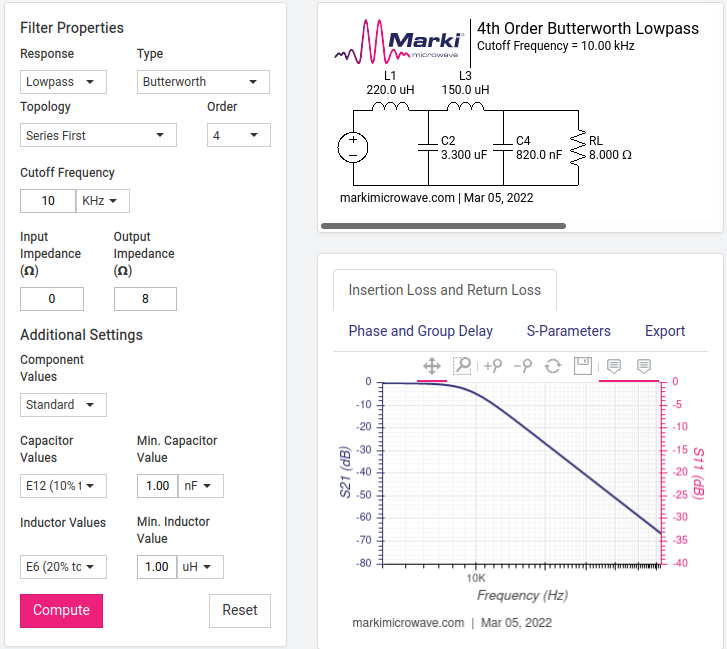
\includegraphics[width=\textwidth]{zvuk-D-butterworth}
    \caption{%
        Návrh filtru pro spínaný zesilovač ve webovém nástroji
        \url{https://rf-tools.com/lc-filter/}
    }
    \label{fig:zvuk D butterworth}
\end{figure}

\begin{figure}[hptb]
    \centering
    \begin{circuitikz}
        \draw
            (0,3) to [L, l=$L_1$, a=$\SI{220}{\micro\henry}$, o-] (3,3)
            to [C, l_=$C_1$, a^=$\SI{3,3}{\micro\farad}$] (3,0)
            to [short, -o] (0,0)
            (3,3) to [L, l=$L_2$, a=$\SI{100}{\micro\henry}$, *-] (6,3)
            to [C, l_=$C_2$, a^=$\SI{1}{\micro\farad}$] (6,0)
            to [short, -*] (3,0)
            (6,3) to [C, l=$C_3$, a=$\SI{220}{\micro\farad}$, *-o] (9,3)
            to [short] (10,3)
            to [loudspeaker, a^=$\SI{8}{\ohm}$] (10,0)
            to [short, -o] (9,0)
            to [short, -*] (6,0)
            (4.5,0) to [short, *-] ++(0,-0.1) node [ground] {}
            ;
    \end{circuitikz}
    \caption{%
        Schéma zapojení filtru pro spínaný zesilovač
    }
    \label{fig:zvuk D filtr sch}
\end{figure}

Umístění vazebního kondenzátoru $C_3$ odstraňujícího stejnosměrnou složku
signálu až na výstup filtru umožňuje použít jako $C_1$ a $C_2$ elektrolytické
kondenzátory, které mají při stejné kapacitě několikanásobně menší rozměry než
například kondenzátory fóliové. Napětí na nich je totiž při normálním provozu
vždy kladné. Vzhledem k malým potřebným kapacitám a provozním napětím ale
postačí i vícevrstvé keramické kondenzátory (MLCC).

Filtr tvořený dvěma cívkami a dvěma kondenzátory má dvě rezonanční frekvence,
při kterých může dojít k nežádoucímu nárůstu napětí na jeho součástkách. Při
připojené zátěži (reproduktor s impedancí \SI{8}{\ohm}) jsou kmity tlumené,
s odpojenou zátěží ale může dojít k výraznému nárůstu napětí například na
kondenzátorech filtru (viz obrázek~\vref{fig:zvuk D filtr sim graf}).



\begin{figure}[htb]
    \centering
    \subcaptionbox{%
        Schéma zapojení a nastavení simulace%
        \label{fig:zvuk D filtr sim sch}
    }{%
        \includegraphics[width=0.80\textwidth]{sim/cropped_zvuk-D-filtr.pdf}
    }
    \subcaptionbox{%
        Útlumová frekvenční charakteristika%
        \label{fig:zvuk D filtr sim graf}
    }{%
        \input{sim/graf-zvuk-D-filtr.tex}
    }
    \caption{Simulace filtru pro spínaný zesilovač v programu LTspice}
    \label{fig:zvuk D filtr sim}
\end{figure}

\FloatBarrier
\paragraph{Bipolární tranzistor jako Zenerova dioda}
V souvislosti s problematikou vysokonapěťových špiček způsobených rezonancí ve
filtru spínaného zesilovače ve stavu odpojené zátěže (reproduktoru) byly
zkoumány metody jejich omezení. K tomuto účelu by byla vhodná Zenerova dioda,
to by ale znamenalo přidání dalšího typu součástky, který je nutné pro osazení
desky plošných spojů opatřit. Za účelem zachování co nejmenšího počtu různých
typů součástek byly prováděny experimenty s použitím běžného bipolárního
tranzistoru NPN, konkrétně jeho přechodu báze--emitor, jako Zenerovy diody.
U křemíkových tranzistorů totiž v závěrném směru dochází k průrazu tohoto
přechodu již od cca \SI{5}{\volt}. Pro účely omezení napěťových špiček
nepotřebujeme, aby napětí průrazu přesně odpovídalo nějaké určité hodnotě.

Pro ověření tohoto konceptu byl vytvořen jednoduchý testovací obvod sestávající
z generátoru funkcí FY6900, který umožňuje dosažení napětí až \SI{25}{\volt},
a~digitálního osciloskopu. Využíváme faktu, že výstupní impedance použitého
generátoru je \SI{50}{\ohm}.

\begin{figure}[htb]
    \centering
    \begin{circuitikz}
        \draw
            (4,3) node [npn] (npn) {BC546}
            (0,3) to [sinusoidal voltage source] (0,0)
            (0,3) to [R=$\SI{50}{\ohm}$] (2,3)
            to [short] (npn.B)
            (npn.E) to [short] (npn.E |- 0,0)
            to [short] (0,0)
            %
            (3,3) to [oscope, *-*] (3,0)
            ;
        \draw[thick, dash dot] (-1,4) rectangle (2.25,-0.5)
            (1,-0.5) node[below] {FY6900}
            ;
    \end{circuitikz}
    \caption{%
        Schéma zapojení obvodu pro testování možnosti využití NPN tranzistoru
        jako Zenerovy diody
    }
    \label{fig:tranzistor zenerka sch testing}
\end{figure}


\begin{figure}[htb]
    \centering
    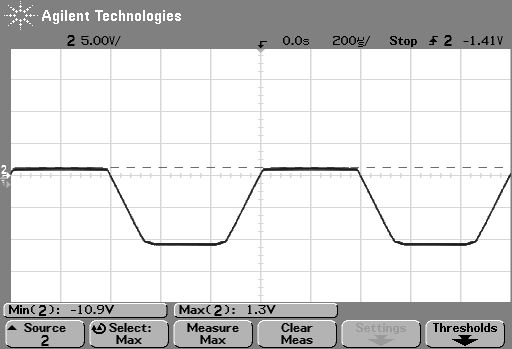
\includegraphics[width=0.8\textwidth]{scope-tranzistor-zenerka}
    \caption{%
        Sinusoida ze zdroje s výstupní impedancí \SI{50}{\ohm} oboustranně
        amplitudově omezená přechodem báze--emitor bipolárního tranzistoru
        BC546
    }
    \label{fig:tranzistor zenerka scope}
\end{figure}

Obvod pracuje dle očekávání, v závěrném směru dochází k nedestruktivnímu
průrazu při napětí \SI{-11}{\volt}. V měřeném rozsahu frekvencí do
\SI{50}{\kilo\hertz} nedochází k žádnému problematickému jevu. Pro výše popsaný
účel by tranzistor postačoval. Zajímavostí je, že simulační program LTspice
(a~programy SPICE obecně) používá model bipolárního tranzistoru, který průraz
přechodu báze--emitor neuvažuje.



\FloatBarrier  % TODO global ??
\subsection{Implementace zvukového výstupu ve firmware}
Generování obdélníkového signálu s určenou periodou je na MCU nejjednodušeji
proveditelné s využitím hardwarové periferie čítače/časovače. V této práci
využitý MCU má těchto periferií několik, pro účely implementace zvukového
výstupu je ale nejvhodnější 16bitový Timer1.

Protože je cílem generovat sinusový signál, musí se perioda PWM signálu v čase
měnit. Toho můžeme dosáhnout periodickým přepisováním hodnoty registru
určujícího střídu. Pro sinusové signály vyšších frekvencí musíme tyto změny
střídy provádět s periodou kratší než jeden průchod hlavní smyčkou. Proto
musíme využít přerušení a hodnotu střídy přepisovat v obslužné rutině ISR.
Toto přerušení potřebujeme spouštět periodicky, tedy při přetečení jednoho
z časovačů. Vhodnou volbou délky běhu časovače Timer1 můžeme dosáhnout toho, že
tento časovač bude vhodný jak pro generování PWM signálu, tak i pro spouštění
ISR.

\subsubsection{Testovací verze}
Pro prvotní ověření konceptu byl vytvořen jednoduchý firmware implementující
pouze zvukový výstup. V repozitáři \gitrepo{AlarmClock} je umístěn v adresáři
\repopath{development/audio}.  % POZOR tuhle cestu mozna zmenim (platformio)

Aby se testovací implementace přiblížila kódu, který by bylo možné zahrnout do
hlavního firmware, je pojata formou knihovny v jazyce \texttt{C} a jednoduchého
Arduino projektu \filename{audio.ino}, který knihovnu využívá.

Hlavičkový soubor \filename{PWMSine.h} definuje API knihovny a je naprosto
triviální:
\begin{lstlisting}[language=C++,style=numbers]
#ifndef PWMSINE_H
#define PWMSINE_H

// PWM period. 20 us (50 kHz) seems to be optimal for further signal
// processing.
#define timer1_us 20

void PWMSine_setup();
void PWMSine_tone(uint8_t pin, uint16_t freq, uint8_t amplitude=255);
void PWMSine_noTone(uint8_t pin);

#endif  // PWMSINE_H
\end{lstlisting}

Knihovna implementuje pouze tři funkce~--
\lstinline[language=C]!void PWMSine_setup()! provádí inicializaci časovače.
\lstinline[language=C]!void PWMSine_tone(uint8_t pin, uint16_t freq, uint8_t amplitude=255)!
zahajuje generování sinusového signálu na výstupním pinu \texttt{pin} (na desce
Arduino UNO jsou použitou knihovnou \texttt{TimerOne} podporované piny 9
a~10~\cite{TimerOnedocs}). Generovaný signál má frekvenci \texttt{freq} a jeho
amplituda je určena 8bitovým číslem \texttt{amplitude}.
\lstinline[language=C]!void PWMSine_noTone(uint8_t pin)! ukončuje generování
tónu na výstupním pinu \texttt{pin}.

Vlastní definice funkcí se nachází v souboru \filename{PWMSine.cpp}:
\begin{lstlisting}[language=C++,style=numbers]
// https://github.com/PaulStoffregen/TimerOne
// version 1.1.0 (git tag 1.1)
#include <TimerOne.h>

#include "PWMSine.h"
#include "sinlut.h"

uint8_t tone_pin;
uint8_t tone_amplitude;
// number of sine wave points per interrupt * 64
// (*64 increases resolution)
uint16_t tone_k;


void timer1_ISR()
{
    static uint16_t i = 0;
    i += tone_k;
    int16_t value = int8_t(pgm_read_byte_near(sin_LUT + (uint8_t)(i/64))) * tone_amplitude / 64;
    Timer1.setPwmDuty(tone_pin, value + 512);
}


void PWMSine_setup()
{
    Timer1.initialize(timer1_us);
    Timer1.stop();
    Timer1.attachInterrupt(timer1_ISR);
}


void PWMSine_tone(uint8_t pin, uint16_t freq, uint8_t amplitude)
{
    tone_k = 64UL * timer1_us * 256UL / (1000000UL/freq);
    tone_pin = pin;
    tone_amplitude = amplitude;
    // Timer1.pwm needs to be called at least once before setPwmDuty can be
    // used.
    Timer1.pwm(tone_pin, 512);
    Timer1.start();
}


void PWMSine_noTone(uint8_t pin)
{
    (void)pin;
    Timer1.stop();
}
\end{lstlisting}

Pro generování PWM signálu je využit 16bitový časovač použitého MCU -- Timer1.
Knihovna \texttt{TimerOne} zprostředkovává jednodušší ovládání této periferie.
Odkaz na její zdrojový kód a specifikace použité verze jsou uvedeny jako
komentář na začátku souboru \filename{PWMSine.cpp}. Jde o svobodnou knihovnu
dostupnou pod podmínkami licence
\foreignlanguage{english}{Creative Commons Attribution 3.0 United States
License}~\cite{TimerOnerepo}.

Funkce \verb|PWMSine_setup| provádí inicializaci časovače a nastavuje periodu
čítání na hodnotu \verb|timer1_us|, tedy \SI{20}{\micro\second}. Poté
zastavuje časovač a nastavuje, aby byla při jeho přetečení zavolána funkce
\verb|timer1_ISR|.

Funkce \verb|PWMSine_tone| nastavuje globální proměnnou \verb|tone_k| na
hodnotu vypočítanou z požadované frekvence sinusového signálu.
Poté nastavuje proměnnou \verb|tone_pin| na hodnotu určenou parametrem
\texttt{pin}. To je nutné, protože tuto hodnotu využíváme ve funkci
\verb|timer1_ISR|. To samé platí pro proměnnou \verb|tone_amplitude|.
Následně zahajuje generování PWM signálu se střídou \SI{50}{\percent} na
výstupním pinu \verb|tone_pin| a zahajuje běh časovače Timer1.

Funkce \verb|PWMSine_noTone| sice přijímá jako parametr výstupní pin,
v současné implementaci ale tuto hodnotu nevyužívá. Aby se zamezilo varování
kompilátoru \shellcmd{gcc} \uv{\foreignlanguage{english}{unused parameter}},
je využita konstrukce jazyka \texttt{C}, která varování při kompilaci potlačí,
ale neprojeví se na generovaném strojovém kódu:
\begin{lstlisting}[language=C]
(void)pin;
\end{lstlisting}
Jediným projevem funkce je tak zastavení časovače Timer1.

Funkce \verb|timer1_ISR| je volána v důsledku hardwarového přerušení,
tedy nezávisle na běhu programu. Protože k tomuto přerušení dochází každých
\SI{20}{\micro\second}, musí mít tato funkce na úrovni strojového kódu co
nejméně instrukcí, aby se minimalizovalo zpomalení běžných operací prováděných
v hlavní smyčce firmware. Funkce při každém zavolání nastavuje 16bitové číslo
$i$ na $i + \mathrm{tone_k}$. Poté určuje výpočtem požadovanou střídu PWM
signálu $\mathrm{value}+512$, kterou nastavuje na používaném časovači. Střída
je 10bitové číslo, nabývá tedy hodnot od \num{0} do \num{1023}. Pro nastavení
střídy PWM signálu je využita metoda \texttt{Timer1.setPwmDuty}, která akci
provede rychleji než \texttt{Timer1.pwm}. \texttt{Timer1.pwm} se ale musí
zavolat alespoň jednou před použitím \texttt{Timer1.setPwmDuty}, protože
provádí inicializaci.~\cite[ověřeno praktickým pokusem]{TimerOnedocs}

Výpočet hodnoty $\mathrm{value}$ určující střídu $\mathrm{value}+512$ pouze
implementuje následující funkci:
\begin{equation}
    d(t) = \num{0,5} + \frac{A}{2} \cdot \sin{(2\pi f t)}
    \label{eq:duty float}
\end{equation}
kde $0 \le d \le 1$ je střída, $f$ je požadovaná frekvence, $0 \le A \le 1$ je
požadovaná amplituda a $t$ je doba uplynulá od začátku generování signálu.

Výpočty s desetinnými čísly s pohyblivou řádovou čárkou by ale byly příliš
pomalé pro použití v ISR, proto jsou využity celočíselné proměnné. Část
výpočtů je též odsunuta do funkce \verb|PWMSine_tone| -- viz proměnná
\verb|tone_k|.

Střída PWM signálu je určena hodnotou funkce $\sin$. Matematické určování
těchto hodnot za běhu programu přímo na MCU by ale bylo příliš časově náročné.
Proto je využita vyhledávací tabulka (LUT) \filename{sinlut.h}, která obsahuje
hodnoty funkce $\sin$ jako 8bitové číslo se znaménkem pro 256 hodnot argumentu
od $0$ do $2\pi$. Tato LUT je generována jednoduchým programem napsaným
v jazyce \texttt{Python}~-- \filename{sinlut.py}~-- spouštěným na standardním
počítači před kompilací firmware:
\begin{lstlisting}[language=Python,style=numbers]
#!/usr/bin/env python3
"""Generate sinlut.h"""

import math

header = """/*!
    @file
    @brief Lookup table for sin.

    This file is automatically generated by `sinlut.py`.
*/

#ifndef SINLUT_H
#define SINLUT_H

const int8_t PROGMEM sin_LUT[] = {
"""

footer = """};

#endif  // SINLUT_H
"""


if __name__ == '__main__':
    with open('sinlut.h', 'w') as f:
        f.write(header)
        for i in range(0, 256):
            value = int(math.sin(2*math.pi / 256 * i) * 127)
            f.write(f'    {value},  // {i}\n')
        f.write(footer)
\end{lstlisting}

Výstupem je soubor \filename{sinlut.h}:
\begin{lstlisting}[language=C++,style=numbers]
/*!
    @file
    @brief Lookup table for sin.

    This file is automatically generated by `sinlut.py`.
*/

#ifndef SINLUT_H
#define SINLUT_H

const int8_t PROGMEM sin_LUT[] = {
    0,  // 0
    3,  // 1
    6,  // 2
    // ...
    -6,  // 254
    -3,  // 255
};

#endif  // SINLUT_H
\end{lstlisting}

Vzorec pro výpočet hodnot funkce $\sin$ pro účely vytvoření LUT je následující:
\begin{equation}
    a(i) = \operatorname{int}\left( \num{127}\cdot\sin{\left(2\pi \cdot \frac{i}{256}\right)} \right)
\end{equation}
kde $\num{-127} \le a \le \num{127}$ je výstupní hodnota pro LUT
a~$\num{0} \le i \le \num{255}$ je pořadí hodnoty $a$ v LUT. Hodnota $a$ je
přetypována na celé číslo ($\operatorname{int}$), desetinná část je tedy
ignorována.

Arduino projekt \filename{audio.ino} je velmi primitivní a pouze využívá funkce
výše popsané knihovny ke generování testovacích signálů:
\begin{lstlisting}[language=C++,style=numbers]
#include "PWMSine.h"

#define pin_speaker 9  // needs to be supported by TimerOne

void setup()
{
    PWMSine_setup();
}


void loop()
{
    PWMSine_tone(pin_speaker, 440, 128);
    delay(1000);
    PWMSine_tone(pin_speaker, 440, 255);
    delay(1000);
    PWMSine_noTone(pin_speaker);
    delay(2000);
}
\end{lstlisting}
Generované signály jsou sinusoida o frekvenci \SI{440}{\hertz} s poloviční
amplitudou po dobu $\SI{1000}{\milli\second} = \SI{1}{\second}$, sinusoida
o frekvenci \SI{440}{\hertz} s plnou amplitudou po dobu \SI{1}{\second} a ticho
po dobu \SI{2}{\second}. Poté se smyčka opakuje.


\subsubsection{Plná verze}
Implementace ve firmware budíku je mírně odlišná. Knihovna \filename{PWMSine.h}
definuje \texttt{C++} třídu \texttt{PWMSine} a její vnitřní kód je v porovnání
s testovací verzí složitější. API knihovny je dokumentováno standardně
technologií \shellcmd{doxygen}.

Oproti testovací verzi přibyla metoda
\lstinline[language=C++]!void PWMSine::silence(uint8_t pin)!, která slouží ke
generování ticha. Kdyby byla místo této metody využita metoda \texttt{noTone},
došlo by k úplnému vypnutí PWM výstupu a výstupní pin by přešel do úrovně
logické~0. To by v reproduktoru způsobilo slyšitelné cvaknutí, protože do té
doby zpracovávaný sinusový signál měl stejnosměrnou složku \SI{2,5}{\volt} a na
tuto hodnotu byl nabit i vazební kondenzátor. Náhlá změna stejnosměrné složky
signálu na \SI{0}{\volt} při vypnutí zvukového výstupu ve firmware se tak na
vstupu lineárního zesilovače (za vazebním kondenzátorem) projeví jako impuls se
špičkou \SI{-2,5}{\volt} -- viz obrázek \vref{fig:zvuk silence sim}. (Poznámka:
ve skutečném obvodu s lineárním zesilovačem je před vazebním kondenzátorem
zařazen atenuátor, takže špička dosahuje pouze zlomku amplitudy
\SI{-2,5}{\volt}. Pro účely vysvětlení tohoto problému ale postačí atenuátor
ignorovat.)

\begin{figure}[htb]
    \centering
    \begin{circuitikz}
        \draw
            (0,3) to [sqV, l=$\SI{1,25}{\volt}$] (0,1.5)
            to [V=$\SI{1,25}{\volt}$] (0,0)
            (0,3) to [short] (2,3)
            to [C=$C_\mathrm{v}$,a=$\SI{100}{\nano\farad}$] (5,3)
            to [R,a=$\SI{1}{\kilo\ohm}$,v^=$u_2$] (5,0)
            to [short] (0,0)
            (2,3) to [open, v^=$u_1$] (2,0)
            ;
    \end{circuitikz}
    \input{sim/graf-zvuk-silence.tex}
    \caption{%
        Schéma zapojení a výsledek počítačové simulace obvodu demonstrujícího
        problémy se cvakáním zvukového výstupu při použití metody
        \texttt{noTone}
    }
    \label{fig:zvuk silence sim}
\end{figure}

Úplné vypnutí zvukového výstupu metodou \texttt{noTone} je sice žádoucí při
ukončení buzení, například během přerušovaného pískání ale působí rušivě.
Objekt \texttt{BuzzerManager} proto v takových případech využívá právě metodu
\texttt{silence}, která na výstupním pinu generuje PWM signál o konstantní
střídě \SI{50}{\percent}.


\paragraph{Příkazy v \texttt{AlarmClockCLI}}
V příkazovém řádku (CLI) budíku byly implementovány příkazy umožňující
jednoduché testování zvukového výstupu. V nápovědě jsou zdokumentovány
následovně:
\begin{lstlisting}[style=terminal]
Help:
  ...
  Sound (testing only):
    tone{f/10};{a}
    silence
    notone
  ...
\end{lstlisting}

Implementace těchto příkazů je velmi jednoduchá. Pokud je firmware zkompilován
s definicí \verb|acite_buzzer|, pouze vrátí chybu \verb|Unsupported|. Pokud je
firmware zkompilován bez této definice, volají příslušné funkce
z~\verb|PWMSine|. Frekvence předávaná příkazu \verb|tone| musí být vydělena 10,
protože v opačném případě by délka tohoto příkazu mohla přesáhnout délku paměti
pro CLI příkazy. Upravit délku paměti by bylo triviální, ale protože jde
o příkaz určený pouze pro testování, bylo zvoleno zkrácení příkazu.

CLI příkazy pro ovládání zvukového výstupu jsou určené pouze pro testování,
protože je s jejich pomocí možné uvést zvukový výstup do stavu, který nelze
s použitím standardních ovládacích prvků opustit.



\paragraph{Melodie}
V průběhu vývoje vyvstal požadavek na možnost změnit frekvenci periodu
a hlasitost přerušovaného pískání při buzení. Vzhledem k jednoduchosti
implementace bylo zvoleno flexibilnější řešení, které umožňuje vytváření
jednoduchých melodií a přiřazování těchto melodií jednotlivým budicím časům.

Melodii můžeme pro účely tohoto projektu definovat jako seznam tónů, které se
postupně přehrávají. Každý tón je charakterizován svou frekvencí, amplitudou
a délkou trvání. Není potřeba definovat speciální případ pro pomlky (období
ticha), protože pro tyto účely můžeme využít tón o libovolné frekvenci
s amplitudou rovnou nule.

Melodie musí být v mikrokontroléru ukládány tak, aby nedošlo k jejich ztrátě
při ztrátě napájení. To vylučuje jejich ukládání v paměti SRAM. Bylo by možné
využít programovou paměť Flash, to by ale vylučovalo jednoduché přepisování
uložených dat za normálního běhu programu (firmware). Proto byla zvolena
interní paměť EEPROM.

Pro ukládání melodií v paměti EEPROM byl vytvořen následující binární formát:
Každá melodie má 3bytovou hlavičku. Hlavička první melodie začíná v EEPROM na
adrese \texttt{0x0010} (definováno konstantou
\verb|EEPROM_melodies_header_start|), následují hlavičky ostatních melodií.
Celkový počet melodií je 16. Hlavička melodie je reprezentována binárními daty
dle následujících pravidel:
\begin{itemize}[nosep]
    \item První byte obsahuje informace o melodii. Jeho nejméně významný bit
        (LSB, bit 0) vždy nabývá hodnoty logické 1. Následující bit nabývá
        hodnoty 1, pokud je melodie aktivovaná. Zbývající bity 2 až 7 jsou
        nevyužité a na jejich hodnotě nezáleží.
    \item Druhý a třetí byte udávají adresu paměti EEPROM, na které začínají
        data dané melodie. Adresa je ukládána jako 16bitové slovo v pořadí bytů
        little-endian.
\end{itemize}

Data melodie začínají 3 byty o hodnotách \texttt{0xFD}; \texttt{0x55};
\texttt{0xAA}. Následuje libovolný počet 3bytových tónů. Data jsou zakončena 3
byty o hodnotě \texttt{0x00}. Validní tón má nenulovou délku trvání, proto se
tato sekvence nemůže vyskytnout uvnitř dat, které ji předchází. Následuje byte
o hodnotě \texttt{0xFF} a 1bytové slovo, jehož LSB je nastaven na 1, pokud se
má po prvním přehrání melodie opakovat. Ostatní bity tohoto slova jsou
nevyužité. Další 3 jednobytová čísla bez znaménka jsou přičtena k amplitudě
všech tónů při 2., 3. a 4. opakování melodie. Třetí číslo je využito i pro 5.
a další opakování. Pokud je amplituda tónu v melodii 0, není toto číslo
přičteno. Pokud je amplituda tónu po přičtení čísla z patičky větší než
\num{255}, je použita hodnota \num{255}, aby se při aritmetické operaci
zabránilo nechtěnému přetečení.

Pokud není patička melodie validní nebo pokud je v hlavičce zapsáno, že melodie
není aktivována, přepne se budík do režimu standardního přerušovaného pípání.
To zajišťuje, že nemůže dojít k tichému přehrávání nevalidních dat.

Každý tón je reprezentován 3 jednobytová čísla bez znaménka:
\begin{itemize}[nosep]
    \item frekvence: $\frac{f - \SI{32}{\hertz}}{\SI{32}{\hertz}}$,
    \item amplituda: \num{0} je ticho, \num{255} je plná hlasitost,
    \item délka trvání: $\frac{t}{\SI{25}{\milli\second}}; t > 0$.
\end{itemize}

Vzorce pro výpočet hodnot uložených v paměti z požadovaných parametrů tónu
vychází z omezení ukládaných čísel na rozsah \numrange{0}{255}.
Vzorec pro přepočet frekvence umožňuje vytváření tónů o frekvencích od
\SI{32}{\hertz} do \SI{8,192}{\kilo\hertz} s rozlišením \SI{32}{\hertz}.
Volba minimální frekvence vychází z původní implementace pomocí funkce \verb|tone|
Volba vzorce pro délku trvání vychází z původního zamýšleného využití
melodií~-- definice vlastního přerušovaného pískání. Je tedy důležité, aby bylo
možné definovat dlouho trvající tóny. Rozsah je \SI{25}{\milli\second} až
\SI{6,375}{\second} s rozlišením \SI{25}{\milli\second}. Podmínka, že délka
trvání tónu nesmí být nulová, umožňuje využít 3 po sobě jdoucí byty s hodnotou
\texttt{0x00} pro zakončení dat v paměti.

Pro testování melodií byly též vytvořeny nové příkazy v CLI:
\begin{lstlisting}[style=terminal]
Help:
  ...
  Melodies:
    melody{i} - play melody 0-15
  EEPROM:
    eer{aaaa} - read data from address
    eew{aaaa};{ddd} - write data to address
  ...
\end{lstlisting}

Příkaz \verb|melody| slouží k zahájení přehrávání vybrané melodie
(\numrange{0}{15}), při použití bez parametru přehrávání ukončuje.
Pro manipulaci s daty v paměti EEPROM byl implementován příkaz
\verb|eer| sloužící ke čtení jednoho bytu z určené adresy a \verb|eew|
provádějící zápis jednoho bytu dat na určitou adresu. Příklad použití nových
příkazů pro práci s daty v EEPROM:
\begin{lstlisting}[style=terminal]
> eer 1023
---
EEPROM:
  1023: 255
...

err 0x0: OK

> eew 1023;10

err 0x0: OK

> eer 1023
---
EEPROM:
  1023: 10
...

err 0x0: OK

> eer 1024

Processing

err 0x1: Invalid args

>
\end{lstlisting}

Pro zjednodušení použití těchto příkazů byl vytvořen program
\shellcmd{acEEPROM} poskytovaný balíčkem \gitrepo{PyAlarmClock}. Ten umožňuje
přečtení souvislého bloku dat z EEPROM a zápis do binárního souboru, nebo
naopak zápis dat z binárního souboru do EEPROM. Například přečtení hlaviček
všech melodií do souboru \texttt{hlavicky.bin} provádíme následovně:
\begin{lstlisting}[style=terminal]
$ acEEPROM /dev/ttyUSB0 read 0x0010 48 hlavicky.bin
INFO:PyAlarmClock:Initializing serial port
100%|#####################| 48/48 [00:03<00:00, 13.09it/s]
$ ls -l hlavicky.bin
-rw-rw-r-- 1 ondra ondra 48 2022-01-07 15:43 hlavicky.bin
$ xxd hlavicky.bin
00000000: 0300 0103 1001 0000 0000 0000 0000 fe00  ................
00000010: 0000 0000 0000 0000 fe00 0000 0000 0000  ................
00000020: 0000 fe00 0000 0000 0000 0000 fe00 0000  ................
$
\end{lstlisting}

Manuální úpravy binárního souboru přečteného z EEPROM jsou zdlouhavé, protože
je nutné neustále nahlížet do dokumentace a dekódovat význam jednotlivých bytů.
Proto je výhodné využít editor binárních dat GNU
\shellcmd{poke}\footnote{\url{http://www.jemarch.net/poke}} implementující
doménově specifický programovací jazyk
Poke\footnote{\url{http://jemarch.net/pokology-01102019.html}}.
Struktura dat je popsána souborem zvaným \texttt{pickle}. Po načtení tohoto
\texttt{pickle} do interaktivního příkazového řádku \shellcmd{poke} provádíme
mapování dané struktury na konkrétní data v binárním souboru a dále s nimi
pracujeme jako s objekty. Celý pickle je uložen v souboru
\repopath{tools/AlarmClockEEPROM.pk} v repozitáři \gitrepo{AlarmClock}, pro
demonstraci konceptu ale použijeme pouze jeho část:
\begin{lstlisting}[language=Poke]
/*
 * Melodies
 */

set_endian(ENDIAN_LITTLE);

type EEPROM_melody_header = struct {
    uint<6>;
    uint<1> enabled;
    uint<1> valid = 1;
    uint<16> data_address;
    method _print = void:
    {
        print "#<\n";
        printf "  enabled: %s\n", enabled ? "yes" : "no";
        printf "  address: 0x%u16x\n", data_address;
        print ">";
    }
};
\end{lstlisting}

Spustíme \shellcmd{poke} a jako parametr mu předáme název binárního souboru~--
\texttt{hlavicky.bin}. Přepínač \texttt{-l} slouží k načtení pickle při
spuštění. Vytvoříme novou proměnnou \verb|melody_headers| jako pole struktur
\verb|EEPROM_melody_header| začínající na začátku souboru (\verb|@ 0#B|). Počet
prvků v poli je určen dynamicky -- prvky se přidávají, dokud se nenarazí na
konec souboru nebo dokud nejde k porušení omezení (\texttt{constraint}).
Protože v našem souboru \texttt{hlavicky.bin} nejsou všechny hlavičky melodií
validní, má pole pouze 2 prvky.
\begin{lstlisting}[style=terminal]
$ poke -l ~/source/repos/AlarmClock/tools/AlarmClockEEPROM.pk hlavicky.bin
     _____
 ---'   __\_______
            ______)  GNU poke 1.0
            __)
           __)
 ---._______)

Copyright (C) 2019-2021 The poke authors.
License GPLv3+: GNU GPL version 3 or later <http://gnu.org/licenses/gpl.html>.
This is free software: you are free to change and redistribute it.
There is NO WARRANTY, to the extent permitted by law.

Powered by Jitter 0.9.258.
Perpetrated by Jose E. Marchesi.

For help, type ".help".
Type ".exit" to leave the program.
+ (poke) var melody_headers = EEPROM_melody_header[] @ 0#B
+ (poke) melody_headers
[EEPROM_melody_header {(uint<6>) 0,enabled=(uint<1>) 1,valid=(uint<1>) 1,data_address=256UH},EEPROM_melody_header {(uint<6>) 0,enabled=(uint<1>) 1,valid=(uint<1>) 1,data_address=272UH}]
+ (poke) .set pretty-print yes
+ (poke) melody_headers
[#<
  enabled: yes
  address: 0x0100
>,#<
  enabled: yes
  address: 0x0110
>]
+ (poke)
\end{lstlisting}
Příkaz \verb|.set pretty-print yes| zapnul uživatelsky přívětivé vypisování,
které volá metody \verb|_print| daných struktur.

S pomocí \shellcmd{poke} bychom mohli například snadno upravit adresu dat
v první hlavičce (\lstinline[language=Poke]|melody_headers[0].address = 0x0123|)
a s pomocí \shellcmd{acEEPROM} binární soubor zapsat zpět do paměti
EEPROM.


\todo[inline]{nekde ukazat postupne zvysovanou amplitudu piskani (scope)}


% Zajimave zdroje (nepouzito, necituji):
% https://uu.diva-portal.org/smash/get/diva2:1219146/FULLTEXT01.pdf
